\subsubsection{Galvanic skin response and temperature data;}
\label{subsubsec:results_gsr_temp_2}

If the variation between the round and the Baseline is positive, it means that the user had an increase on his/her Mental Workload or stress. While the GSR varied for the blind participants, increasing for methods with vibration, the same does not happen for sighted participants. Also, the variance of GSR data for blind participants is significantly higher than that of sighted ones. The same conclusion can be drawn from the boxplots in Figures \ref{fig:boxplot_ecg_sdnn_4_scene} and \ref{fig:boxplot_ecg_sdnn_4_rounds}. 

\begin{figure}[!htb]
    \centering
    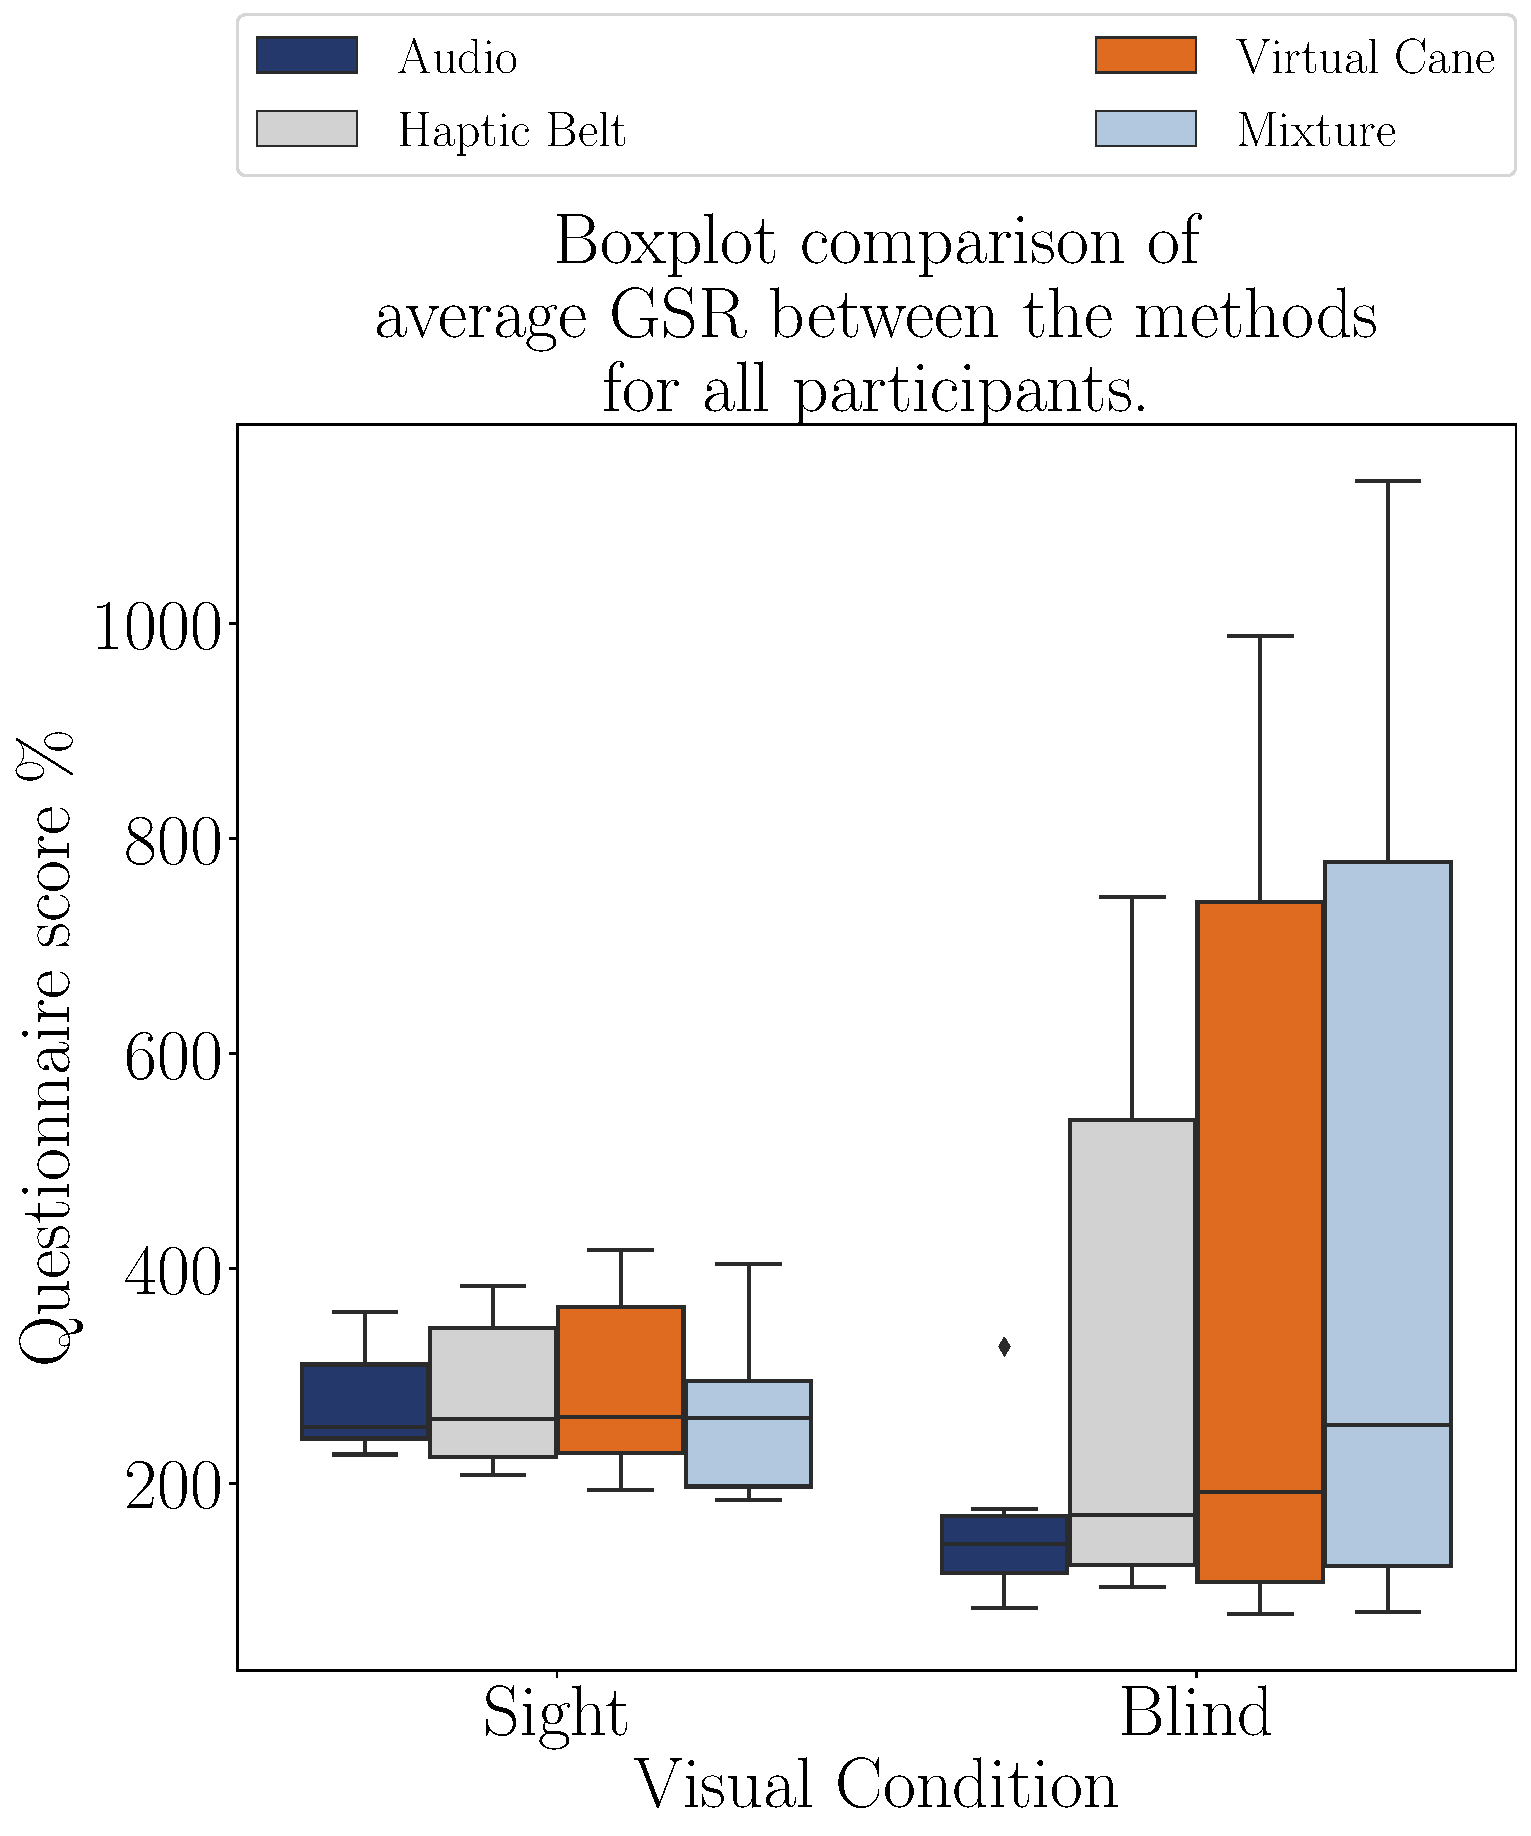
\includegraphics[width = 0.75\linewidth]{3 - Resultados/Figuras/boxplot_gsr_avg_4_scene.pdf}
    \caption{Boxplot of the average GSR of the participants grouped by method.}
    \label{fig:boxplot_gsr_avg_4_scene}
\end{figure}
\begin{figure}[!htb]
    \centering
    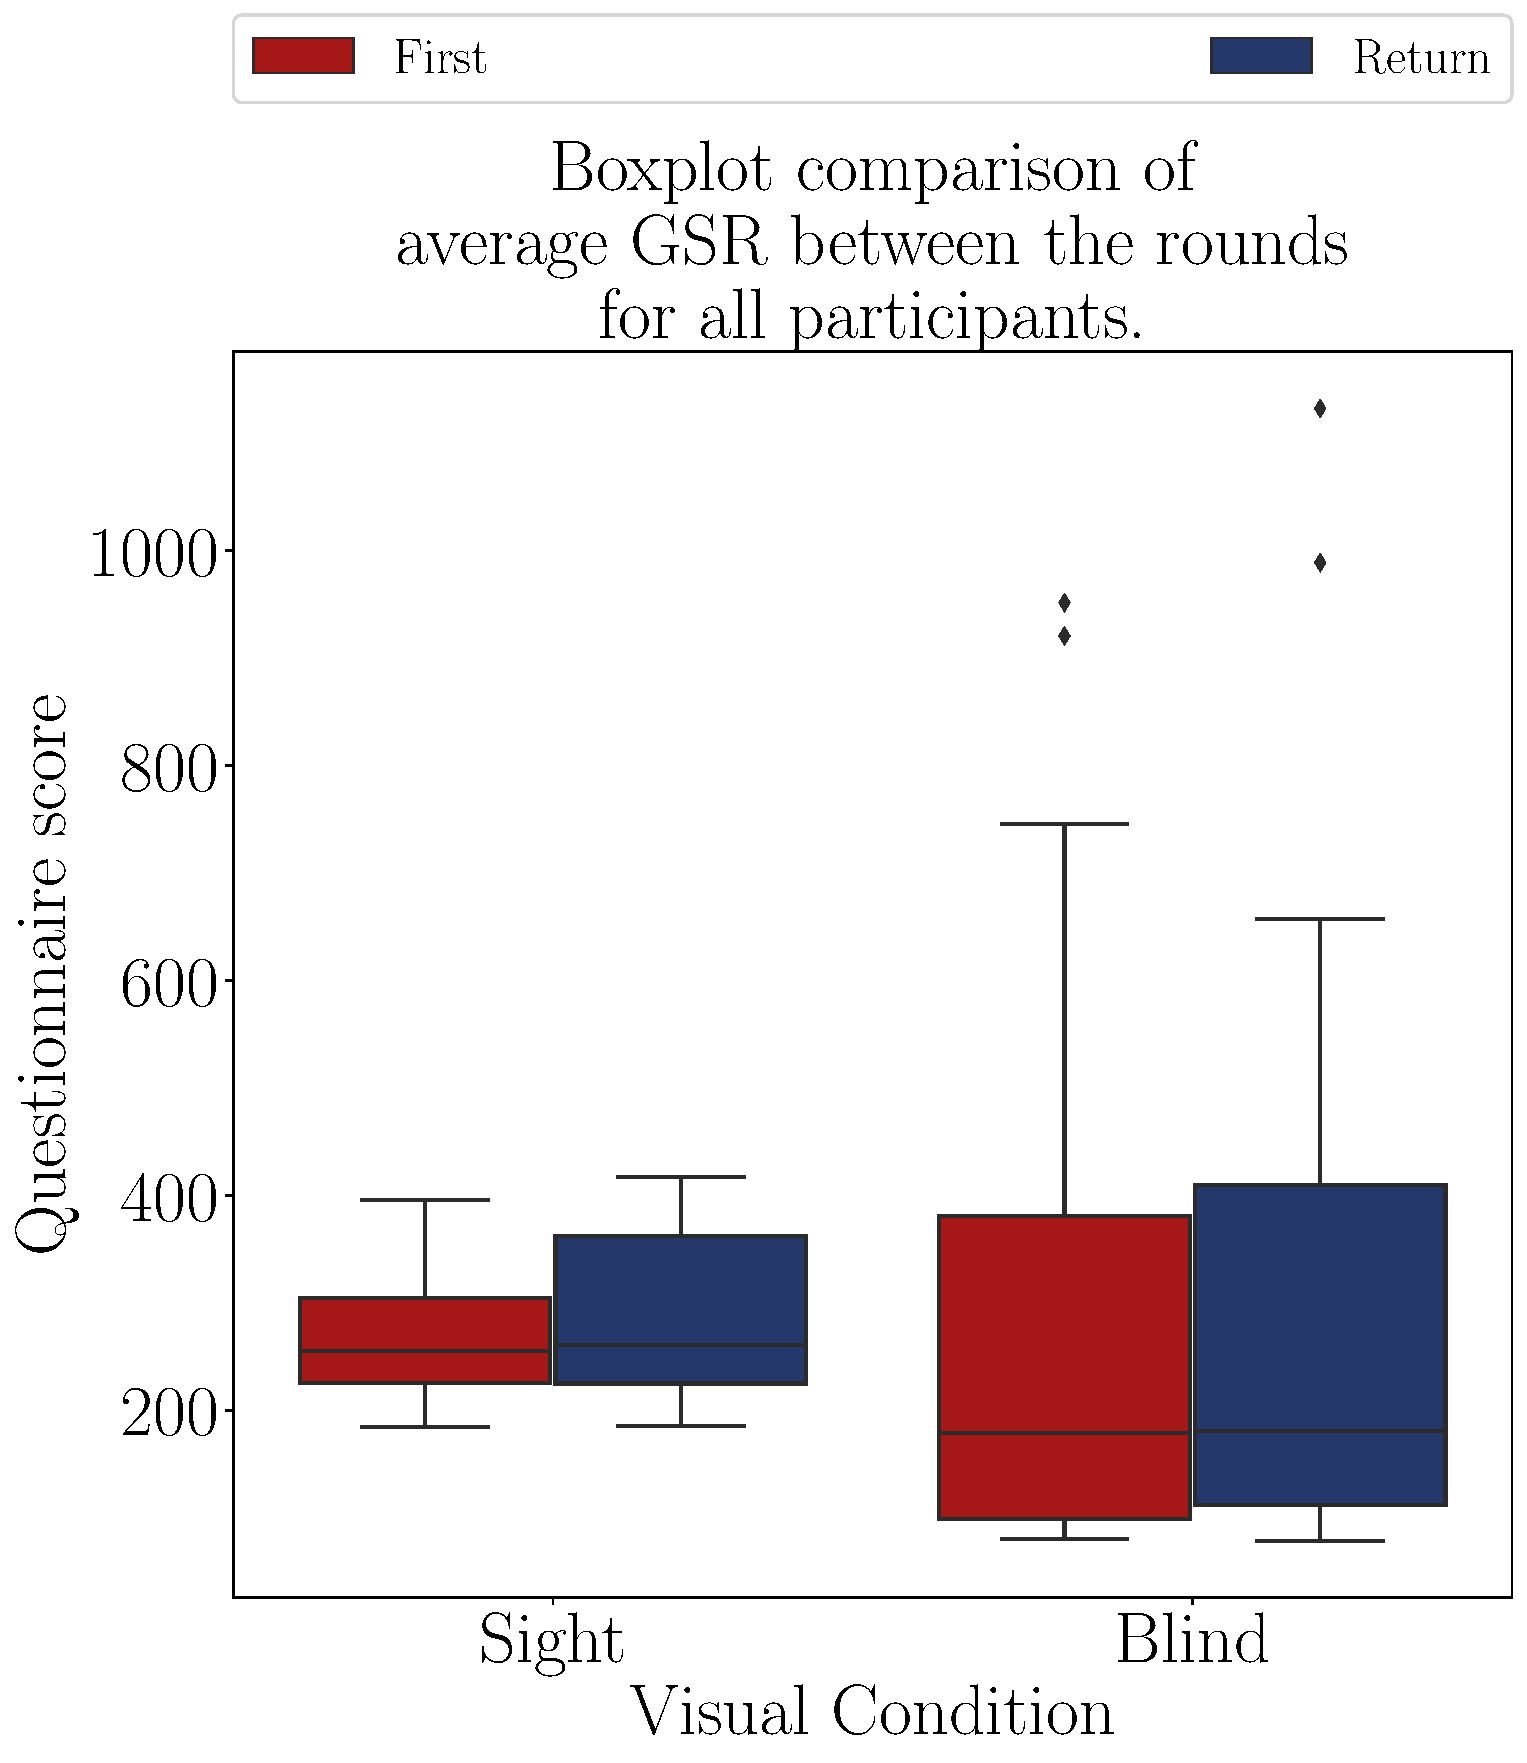
\includegraphics[width = 0.75\linewidth]{3 - Resultados/Figuras/boxplot_gsr_avg_4_rounds.pdf}
    \caption{Boxplot of the average GSR of the participants grouped by round.}
    \label{fig:boxplot_gsr_avg_4_rounds}
\end{figure}

The results from ANOVA are presented in Table \ref{tab:blocanova_gsr_two_way_blind_sight}. In the case of blind participants, the p-value for the method is just slightly over the threshold, indicating a possible influence of the method. The same does not happen with sighted participants, where the p-value of the method factor is the highest and well above the 0.05 threshold.

\begin{table}[!htb]
    \caption{Anova p-value for the skin conductance average on each method}
    \label{tab:blocanova_gsr_two_way_blind_sight}
\begin{minipage}{0.45\linewidth}
    \subcaption{Blind participants}
    \input{3 - Resultados/Tabelas/blocanova_gsr_two_way_blindsemBegin.tex}
\end{minipage}%
\begin{minipage}{0.05\linewidth}
    \hfill
\end{minipage}%
\begin{minipage}{0.45\linewidth}
    \subcaption{Sight participants}
    \input{3 - Resultados/Tabelas/blocanova_gsr_two_way_sightsemBegin.tex}
\end{minipage}
\end{table}